\documentclass{article}
\usepackage[utf8]{inputenc}
\usepackage{amsmath, dsfont, mathtools}
\usepackage{graphicx, float}
\usepackage[most]{tcolorbox}
\usepackage{enumitem}
\usepackage{hyperref}
\usepackage{tikz}
\usepackage{xcolor}

% ------------------------------------ %
%             Customization            %
% ------------------------------------ %

\usepackage[letterpaper, top=1in, left=1in, right=1in, bottom=1in]{geometry}
\setlength{\parindent}{0em}
\setlength{\parskip}{0.5em}
\setlist[enumerate]{itemsep=-0.5em} % Adjust the spacing as desired
\setlist[itemize]{itemsep=-0.5em} % Adjust the spacing as desired
\renewcommand{\baselinestretch}{1.25}

\title{MATH1853}
\author{Jax T}
\date{23 Dec}

\newtcolorbox{knBox}[2][]{
arc=2mm, 
lower separated=true, % Set to true to enable the separation between upper and lower sections
segmentation style={dashed, draw=black}, % Add dashed line style between the sections
fonttitle=\bfseries,
colbacktitle=white!10,
coltitle=black,
enhanced,
attach boxed title to top left={xshift=0.2cm,
        yshift=-2mm},
colframe=white!40!black,
boxrule=0.3mm,
colback=black!02,
title=#2,#1
}

\newtcolorbox{defBox}[2][]{
arc=2mm, 
lower separated=true, % Set to true to enable the separation between upper and lower sections
segmentation style={dashed, draw=black}, % Add dashed line style between the sections
fonttitle=\bfseries,
colbacktitle=green!10,
coltitle=black,
enhanced,
attach boxed title to top left={xshift=0.2cm,
        yshift=-2mm},
colframe=green!40!black,
boxrule=0.3mm,
colback=green!02,
title=#2,#1
}

\hypersetup{
    colorlinks=true,
    linkcolor=purple    % Color for internal links
}

\newenvironment{amatrix}[1]{%
  \left[\begin{array}{@{}*{#1}{c}|c@{}}
}{%
  \end{array}\right]
}

\newcommand{\note}[1]{\textcolor{gray}{\tiny #1}}

% ------------------------------------ %
%              Title page              %
% ------------------------------------ %
\begin{document}

\begin{titlepage}
    \null\vfill % Add vertical space to center the title and author
    
    \centering
    \Huge\textbf{MATH1851}
    
    \vspace{0.1cm}
    \Large\textbf{Notes Spring 2024}
    
    \vspace{1cm}
    \normalsize\textbf{Author:} Jax
    
    \normalsize\textbf{Contact:} enhanjax@connect.hku.hk
    \vfill % Add vertical space to center the remaining space
\end{titlepage}

% ------------------------------------ %
%               Document               %
% ------------------------------------ %

\section{Limits and Continuity}
\begin{defBox}[]{Average rate of change}
  \begin{flalign*}
    \frac{\Delta y}{\Delta x}&=\frac{f(x_1+h)-f(x_1)}{h},\quad\text{for }x_2=x_1+h,h\ne 0&
  \end{flalign*}
\end{defBox}

\subsection{The concept of limit}
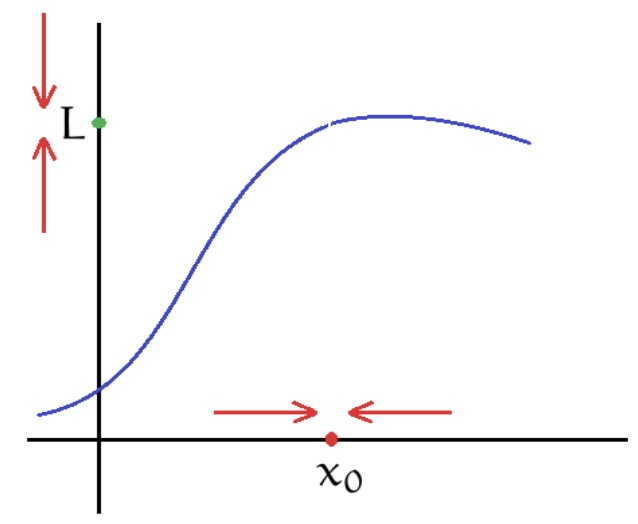
\includegraphics[width=0.2\textwidth]{img/Lim.jpg}

The limit of $\lim_{x\to x_0}f(x)$ exists if the value of $f(x)$ gets close to $L$ as $x_0$ gets close to $x$. Therefore, $\lim_{x\to x_0}f(x)=L$. However, \emph{the limit of a function may or may not exist}.

For a positive example, $\lim_{x\to x_0}x=x_0$.

However, if the value is \emph{different} when $f(x)$ gets close to the limit from either side, we say that the limit \emph{does not exist}.

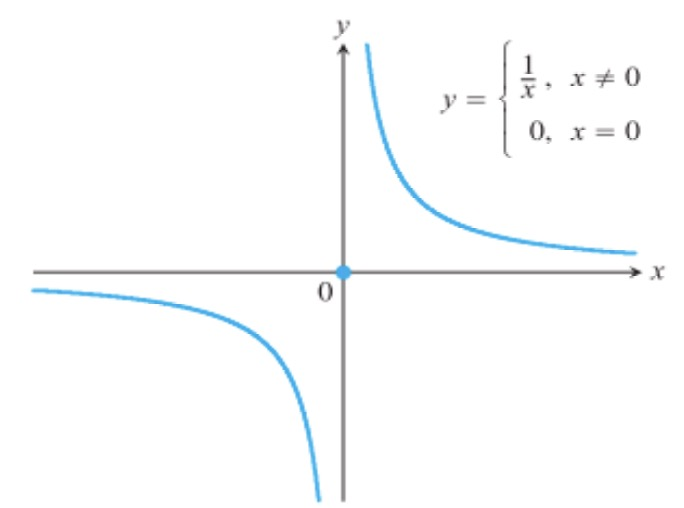
\includegraphics[width=0.2\textwidth]{img/lim3.jpg}

As $x\to(\text{tends to})\ 0$ from the left, which means the same as $x\to 0^-$, $y\to -\infty$. Similarly, as $x\to 0^+, y\to +\infty$.

As they tend to a different number when getting close to the same point, $\lim_{x\to 0}y$ doesn't exist.

\subsection{Techniques}
\subsubsection{Limit Laws}

\end{document}